\documentclass[../main]{subfiles}

\input{chapter_header.tex}

\begin{document}

% TikZ styles
\tikzset{
    block/.style={
        rectangle,
        draw,
        rounded corners=3pt,
        align=center,
        minimum height=1cm,
        minimum width=2.8cm,
        fill=blue!8
    },
    arrow/.style={
        -{Stealth[length=3mm, width=2mm]},
        thick
    }
}

\chapter{SINC: System Design and Implementation}

The Seed Incubation Environmental Control System integrates hardware,
communication protocols, and software interfaces to maintain optimal conditions
for seed growth. The system ensures continuous monitoring, precise actuation,
and remote control through a user-friendly mobile interface.

\section{System Architecture}

The system architecture is structured into three layers: hardware,
communication, and software. The hardware layer comprises the ESP32
microcontroller and sensors. Data from sensors is transmitted via the MQTT
protocol to the Flutter application, forming the software layer. Users can view
live data, adjust thresholds, and receive alerts when conditions deviate. This
layered approach ensures modularity, scalability, and reliable operation.

\section{Working Principle}

Sensors continuously measure environmental parameters. The ESP32
microcontroller processes these readings and publishes them to MQTT topics
hosted on a broker. The Flutter application subscribes to these topics,
updating the interface in real-time. When a parameter exceeds its threshold,
the ESP32 actuates devices to restore conditions, achieving a fully automated
closed-loop system.

\begin{figure}[H]
\centering
\vspace{0.25cm}
    \begin{tikzpicture}[
            scale = 0.55,
            transform shape,
            node distance=1.4cm and 2cm
        ]

        % Top Layer
        \node[block] (app) {SINC App};
        \node[block, below=1.0cm of app] (ui) {User Interface};

        % Second Layer
        \node[block, below left=1.5cm and 2.0cm of ui] (home) {Home / Overview Page};
        \node[block, below=of ui] (controlcenter) {Control Center};
        \node[block, below right=1.5cm and 6.5cm of ui] (incsettings) {Incubator Settings};

        % Third Layer
        \node[block, below=1.0cm of home] (overview) {Overview of the Incubator};
        \node[block, below=of controlcenter] (widgets) {List of Widgets};
        \node[block, below=1.0cm of incsettings] (rawcontrols) {Raw Controls};

        % Fourth Layer
        \node[block, below left=1.8cm and 0.5cm of widgets] (temphum) {Temperature and Humidity};
        \node[block, below right=1.8cm and 0.5cm of widgets] (lighting) {Lighting};
        \node[block, below=1.0cm of rawcontrols] (actuator) {Actuator Control};

        % Fifth Layer
        \node[block, below left=3.8cm and -0.75cm of widgets] (peltier) {Peltier Control};
        \node[block, below right=3.8cm and -0.75cm of widgets] (humidifier) {Humidifier Control};
        \node[block, below left=1.4cm and -1.1cm of actuator] (panelmotors) {Panel Motors Control};
        \node[block, below right=1.4cm and -0.8cm of actuator] (hatchmotors) {Hatch Motors Control};

        % Connections
        \draw[arrow] (app) -- (ui);
        \draw[arrow] (ui) -- (home);
        \draw[arrow] (ui) -- (controlcenter);
        \draw[arrow] (ui) -- (incsettings);

        \draw[arrow] (home) -- (overview);
        \draw[arrow] (controlcenter) -- (widgets);
        \draw[arrow] (incsettings) -- (rawcontrols);

        \draw[arrow] (widgets) -- (temphum);
        \draw[arrow] (widgets) -- (lighting);
        \draw[arrow] (rawcontrols) -- (actuator);

        \draw[arrow] (widgets) -- (peltier);
        \draw[arrow] (widgets) -- (humidifier);
        \draw[arrow] (actuator) -- (panelmotors);
        \draw[arrow] (actuator) -- (hatchmotors);

    \end{tikzpicture}
\caption{Working principle diagram of the Seed Incubation Control System}
\end{figure}

\section{MQTT Communication Protocol}

The MQTT protocol provides lightweight, efficient communication between the
ESP32 and the mobile app. Following a publish-subscribe model, the ESP32
publishes sensor readings to topics, while the app subscribes to receive these
updates. This approach ensures minimal latency, reduces bandwidth requirements,
and allows multiple devices to communicate simultaneously through the broker.
Persistent connections ensure that no data is lost, even in fluctuating network
conditions.

\section{App Design and User Interface}

The Flutter app was designed to provide clear visualization of environmental
data and intuitive controls. The Home screen displays live sensor readings,
graphs, and alerts. Detailed pages for each parameter show historical trends
and current values. The Settings screen allows users to adjust thresholds and
configure alerts. Smooth navigation transitions and iconography enhance user
experience.

\begin{tabular}{cccc}
\vspace{0.5cm}
    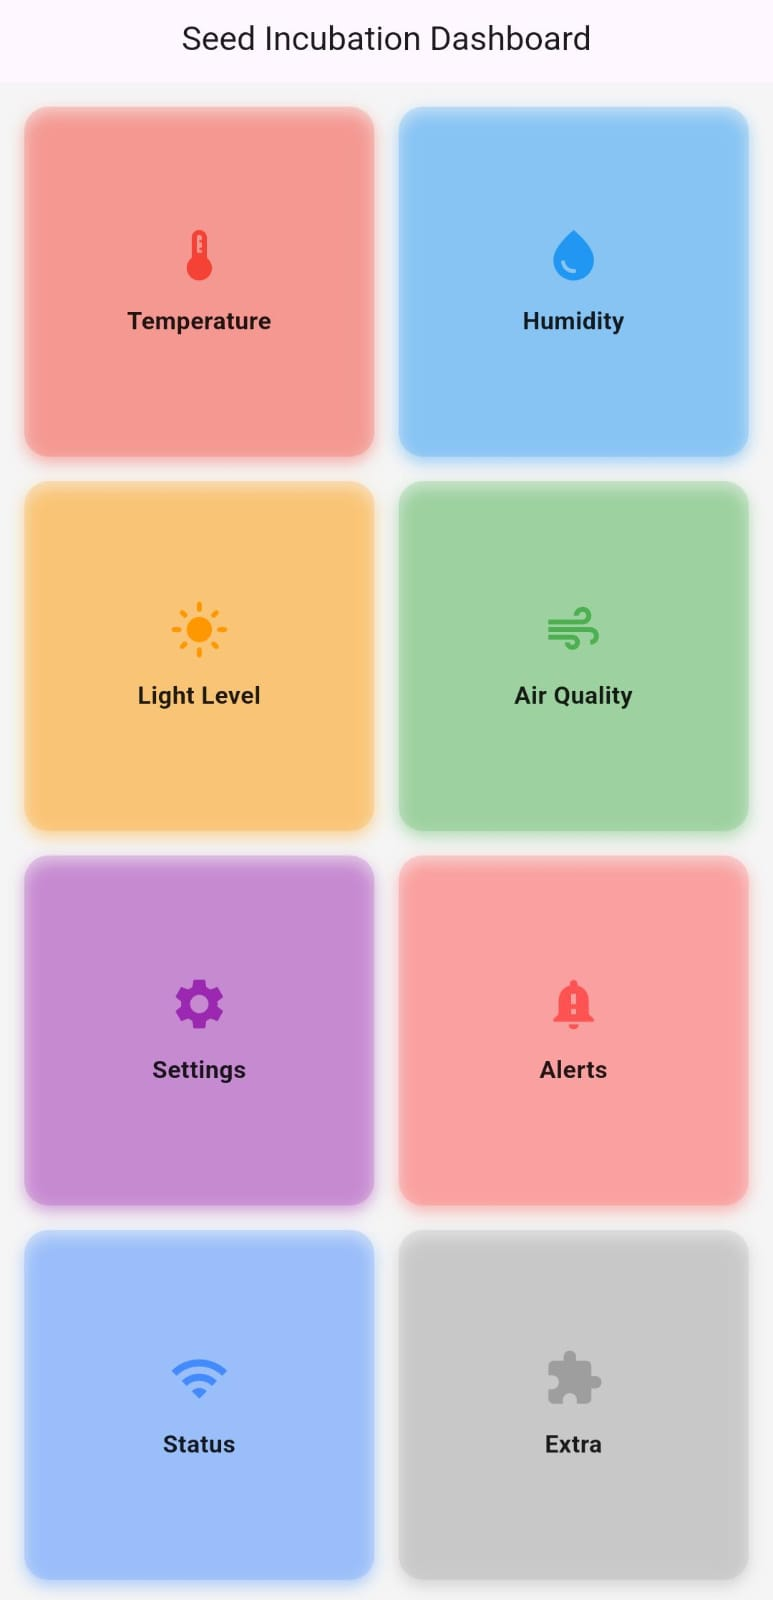
\includegraphics[width=0.22\textwidth]{pics/app4.jpeg} &
    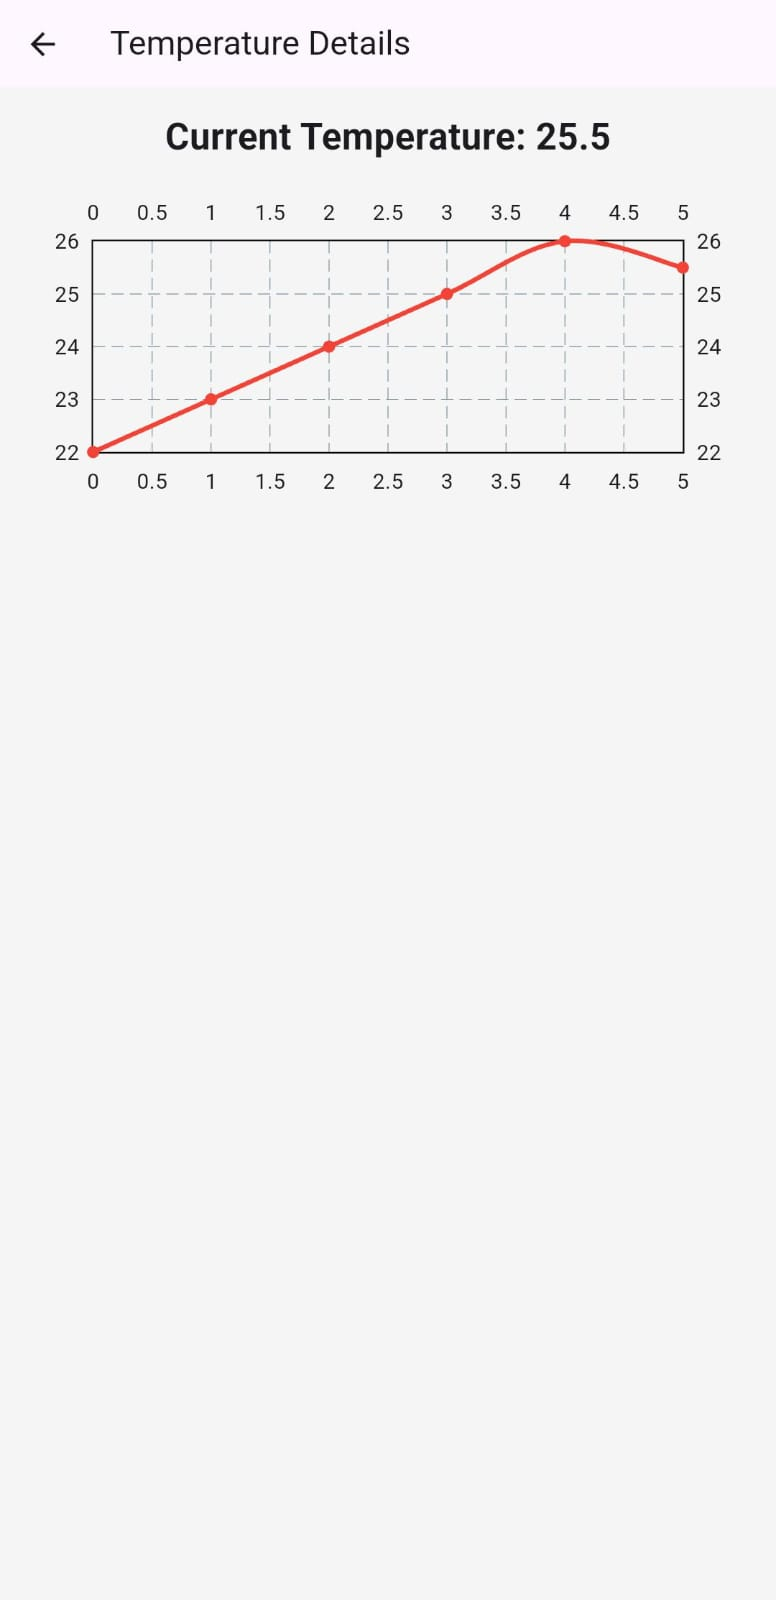
\includegraphics[width=0.22\textwidth]{pics/app5.jpeg} &
    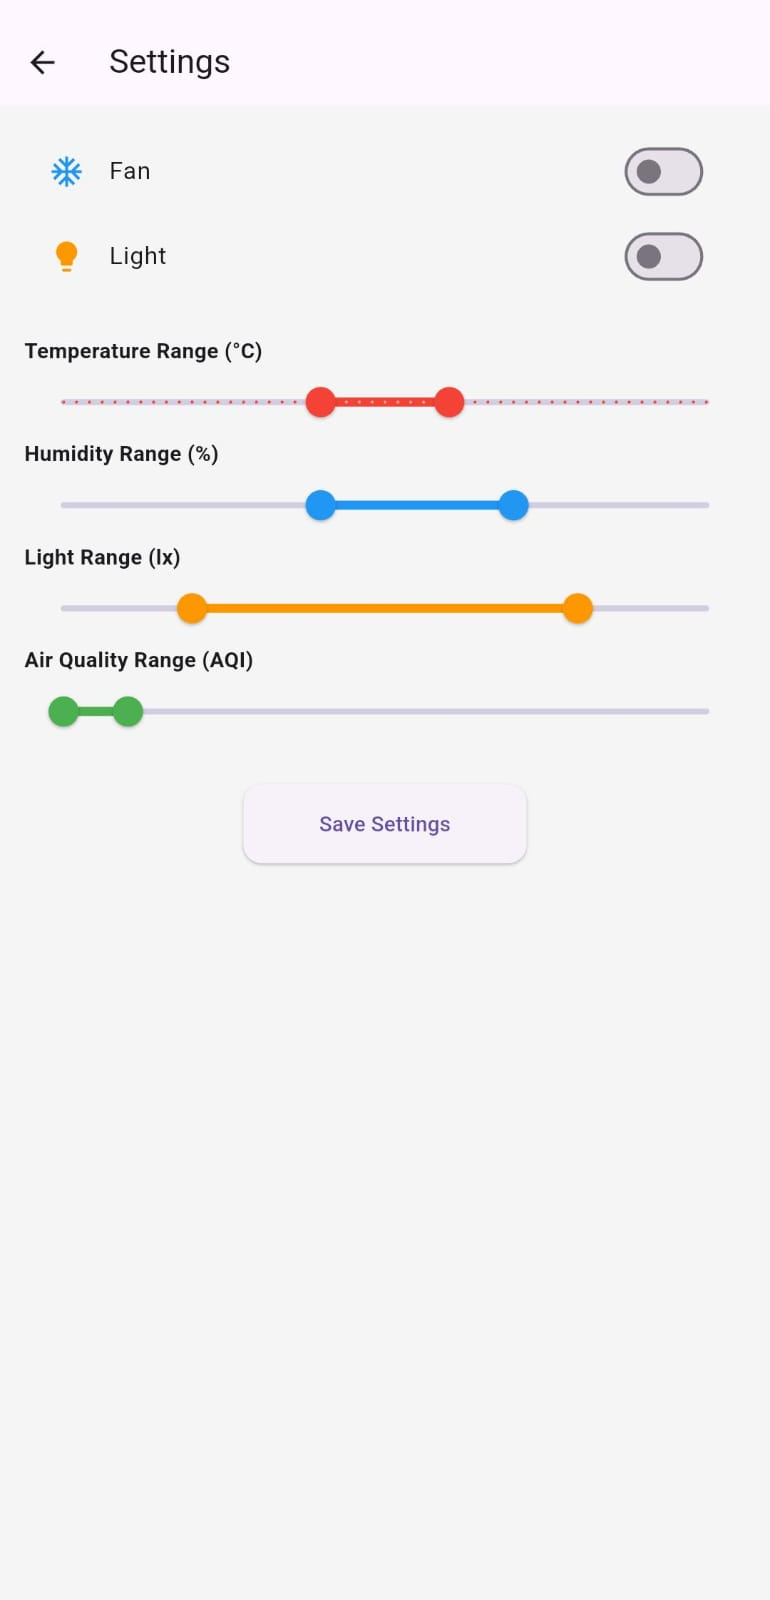
\includegraphics[width=0.22\textwidth]{pics/app2.jpeg} &
    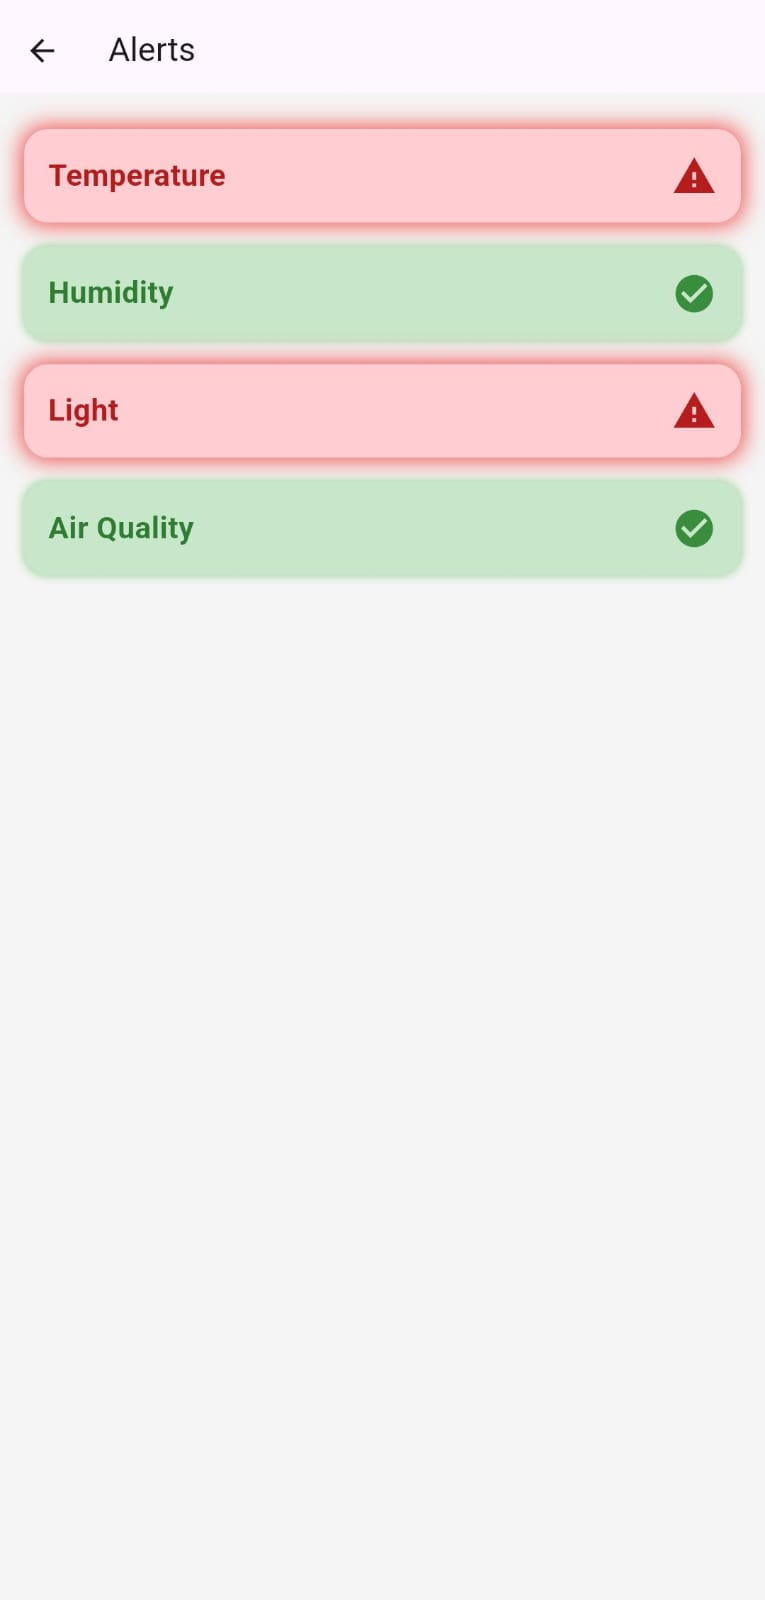
\includegraphics[width=0.22\textwidth]{pics/app6.jpeg} \\
    \textbf{Home} & \textbf{Status} & \textbf{Settings} & \textbf{Alerts} \\
\end{tabular}

\section{Navigation Flow and Control Logic}

The navigation within the app is straightforward. The splash screen introduces
the application, followed by the Home dashboard. Users can access
parameter-specific detail pages, charts, and the Settings section to adjust
control limits. Each user interaction triggers immediate MQTT communication,
ensuring the physical system responds in real-time to app commands. This
event-driven logic maintains closed-loop control without delays.

\section{Software and Hardware Implementation}

The mobile app is developed in Flutter with the Dart programming language,
enabling real-time updates and cross-platform deployment. Sensors continuously
monitor environmental parameters, while actuators such as heaters, fans, and
humidifiers respond instantly to threshold breaches, completing the automated
feedback loop.

\section{Advantages of the System}

The integrated system provides automated control, continuous monitoring, and
remote accessibility. By minimizing human intervention, it reduces errors and
labor requirements. Users gain actionable insights through real-time data
visualization and can adjust conditions as needed, making the incubation
process more reliable and efficient. The system’s modular design supports
scalability and future feature expansion.

\section{Future Enhancements}

Future improvements include cloud-based data storage for long-term tracking,
AI-assisted predictive control, voice command integration, multi-device
support, and adaptive controls based on environmental trends. These
enhancements will further increase intelligence, usability, and efficiency,
solidifying the system as a comprehensive tool for modern seed incubation
management.

\section{Conclusion}

The Seed Incubation Environmental Control App successfully demonstrates the
combination of IoT, mobile computing, and automation for precision agriculture.
The system delivers accurate monitoring, remote control, and automated
actuation, ensuring optimal conditions for seed growth. This project
contributes to advancing smart agricultural practices, reducing labor, and
increasing efficiency in controlled environment agriculture.

\end{document}
